\chapter{From \$0 to \$12M a Year at Twenty-Six}

These notes follow a School of Hard Knocks interview, curated by LazyingArt LLC, and treat it as a compact lecture on entrepreneurial scale. The central question is simple enough to state and hard enough to matter: how does one move from zero, or from a modest six-figure business, to a level where million-dollar thresholds stop feeling mystical and become operational? The chapter therefore follows the order of the interview itself: first the stakes, then the first business, then the arithmetic of scale, then sales, network, reinvestment, discipline, and finally the problem of rebuilding from zero.

\begin{remark}
No blackboard equations survive from this lecture. The displayed formulas below are careful transcript-based reconstructions of Victor's spoken business logic rather than transcriptions of visible board work.
\end{remark}

\section{Opening Stakes}

The lecture begins with a compressed biography. Victor is introduced as someone who, over roughly six years, moved from an empty bank account at age nineteen to a net worth above ten million dollars at age twenty-six. The interviewer adds a present-day revenue marker as well: halfway through the current year, Victor says he is at six million dollars. These are not audited balance-sheet statements; they are the scale markers that motivate everything that follows.

\begin{align}
R_{\text{half-year}} &\approx \$6{,}000{,}000, \\
\mathrm{NW}_{26} &> \$10{,}000{,}000.
\end{align}

The important thing is not merely the size of these numbers. The important thing is the question they generate. The interviewer frames the whole discussion around the move from an ordinary entrepreneurial beginning to a level where a one-million-dollar target, and then a ten-million-dollar target, can be handled without paralysis. That question will later be answered by arithmetic, cadence, and positioning rather than by mystique.

\section{E-Commerce as Attention Arithmetic}

The first business named in the interview is an e-commerce clothing brand. This is the first local case from which Victor extracts a general rule.

\paragraph{Anecdote.}
In a crowded apparel market, he did not wait for the perfect drop. He says he released clothes every week, and sometimes twice a week, whether the result was good, bad, or commercially impressive.

\paragraph{Claim.}
The immediate problem is not abstract quality. The immediate problem is attention. Social media is full of distractions, and a six-month perfection cycle easily disappears from public memory.

\paragraph{Mechanism.}
What matters, in the language of these notes, is repeated exposure. If we let \(f_{\text{drop}}\) denote release frequency and \(E\) denote audience exposure, then the interview suggests the directional relation
\begin{equation}
E \uparrow \quad \text{as} \quad f_{\text{drop}} \uparrow.
\end{equation}
This is not a measured law. It is a disciplined shorthand for the spoken claim that repeated drops keep the brand in front of people until the brand becomes normal in their feed.

Schematically, the contrast is
\begin{align}
f_{\text{drop}}^{\text{Victor}} &\in \{\text{weekly},\ \text{twice weekly}\}, \\
f_{\text{drop}}^{\text{slow launch}} &\approx \text{once per six months}.
\end{align}

The argument is subtle. He is not claiming that every drop succeeds. He is claiming that frequency changes the background field in which success becomes possible. The brand is seen more often; repeated appearance reduces novelty and increases familiarity; familiarity changes the odds that the next offer is not ignored. That is the first piece of mathematics in the lecture: not calculus, but cadence.

\section{The Game of Numbers}

The interview now widens from one clothing brand to the general problem of scaling from six figures to seven. Here we reach the lecture's cleanest quantitative moment.

\begin{definition}
By the \emph{game of numbers} we mean the practice of replacing a frightening aggregate target \(T\) by a repeatable unit \(u\) and a repetition count \(n\), so that
\begin{equation}
T = u \cdot n.
\end{equation}
\end{definition}

Victor also uses the phrase ``game of doubles,'' but the arithmetic example he actually gives is a repeated-ten ladder rather than literal doubling. We should preserve the phrase, but the structure is clear enough: the mind should stop staring at the final figure and begin working with manageable units.

\subsection{A Worked Example}

He explicitly decomposes the million-dollar target in two steps:
\begin{align}
\$10{,}000 \times 10 &= \$100{,}000, \\
\$100{,}000 \times 10 &= \$1{,}000{,}000.
\end{align}
Combining the two steps gives
\begin{equation}
\$10{,}000 \times 10 \times 10 = \$1{,}000{,}000.
\end{equation}

We should pause here, because this is the lecture's main calming device. The target is not removed; it is factorized. The speaker's point is that a million-dollar aspiration becomes operational once it is rewritten as a chain of smaller wins.

The logic can be written as a short derivation:
\begin{enumerate}
\item Start with the intimidating target \(T=\$1{,}000{,}000\).
\item Refuse to treat \(T\) as one indivisible event.
\item Rewrite it as ten instances of \(\$100{,}000\).
\item Rewrite each \(\$100{,}000\) block as ten instances of \(\$10{,}000\).
\item Therefore the path to \(T\) is not one leap but repeated execution of a smaller unit.
\end{enumerate}

\begin{figure}
\centering
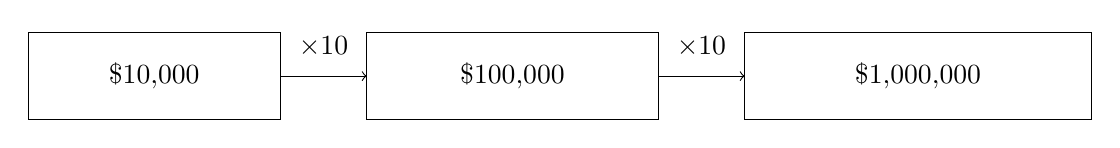
\begin{tikzpicture}
\draw (0,0) rectangle (3.2,1.1);
\node at (1.6,0.55) {$\$10{,}000$};

\draw (4.3,0) rectangle (8.0,1.1);
\node at (6.15,0.55) {$\$100{,}000$};

\draw (9.1,0) rectangle (13.5,1.1);
\node at (11.3,0.55) {$\$1{,}000{,}000$};

\draw[->] (3.2,0.55) -- (4.3,0.55);
\node at (3.75,0.92) {$\times 10$};

\draw[->] (8.0,0.55) -- (9.1,0.55);
\node at (8.55,0.92) {$\times 10$};
\end{tikzpicture}
\caption{Victor's scaling ladder: the target is handled one figure at a time.}
\end{figure}

After giving this arithmetic, Victor adds a second claim: he did not rely on ad spend to propel the work. The operative verb is ``show up.'' So the formal ladder above is not a substitute for repetition; it is a way of making repetition thinkable. The million-dollar figure ceases to be a monument and becomes a schedule.

\section{Sales as Positioning}

Once the lecture has decomposed scale into repeated units, the next live question is obvious: how does one convert the marginal client who is leaning toward no?

\subsection{Question \& Answer}

\paragraph{Question.}
Suppose a prospective client or customer is on the fence and drifting toward refusal. What is the right move if the aim is to turn a no into a yes?

\paragraph{Answer.}
Victor's answer is strikingly negative: do not push. Pressure creates the wrong inference. The buyer reads repeated insistence as evidence that the seller needs the deal more than the deal needs the buyer. In the notation of these notes, if \(P_{\text{push}}\) denotes the intensity of overt pressure, then the interview suggests the directional claim
\begin{equation}
P_{\text{push}} \uparrow \;\Rightarrow\; \Pr(\text{resistance}) \uparrow.
\end{equation}

The positive side of the argument is just as important. The goal is to become so good, and so visibly established, that people come inward rather than needing to be chased. This is a status-and-scarcity model of sales rather than a pressure model. One does not merely persuade; one changes the geometry of the transaction.

A compact transcript-based rendering is
\begin{equation}
\text{quality} + \text{scale} + \text{scarcity} \;\Rightarrow\; \text{inbound demand}.
\end{equation}

The interview immediately gives a concrete business mechanism for this. Victor says that the business was scaled into an elite program, and that there was a paid subscription allowing some customers to enter the website earlier than everybody else. The principle is clear: scarcity is not merely emotional posture; it can be operationalized as paid early access. The sale is strengthened when the offer is not universally and instantly available.

\section{Network as Leverage}

After sales, the lecture broadens its scope. We move from transaction-level behavior to the environment in which ambition is measured. Victor says that, besides consistency, network is crucial because one becomes a product of one's environment.

The claim here is not decorative. The right room changes the benchmark. If the people around us are operating above our present level, then our own horizon is stretched. If they are operating below it, then early success can feel terminal.

\paragraph{Claim.}
Network is treated as a multiplier of standards rather than as a pleasant social accessory.

\paragraph{Mechanism.}
The comparison class changes the sense of what is normal. A room full of people doing more than we are doing destroys complacency. A room full of people doing less can create the illusion that the work is finished.

\subsection{Question \& Answer}

\paragraph{Question.}
What if one accepts the importance of network but has not yet gained access to those rooms? How does one enter without merely asking for rescue?

\paragraph{Answer.}
The answer is to enter with value. One sharpens a skill until it becomes legible as a missing piece in someone else's system. In that language, if \(S_{\text{offer}}\) denotes the strength of the value one can bring, then
\begin{equation}
S_{\text{offer}} \uparrow \;\Rightarrow\; \Pr(\text{access}) \uparrow.
\end{equation}

The transcript describes this with the image of a puzzle piece. Someone else may have more money and more success, but if we bring the one capability they lack, we do not enter as a supplicant. We enter as a complement.

The logic can be laid out cleanly:
\begin{enumerate}
\item Invest in oneself first.
\item Build a skill until it is concrete and usable.
\item Identify a gap in the stronger person's business.
\item Offer the missing piece rather than requesting generic help.
\item Convert access from charity into exchange.
\end{enumerate}

This is a hard idea, but it has the right flavor. The room opens not because one deserves encouragement, but because one reduces somebody else's deficiency.

\section{Asset Logic, Time Discipline, and the Restart from Zero}

The lecture now compresses several principles into rapid succession. The key is not to flatten them. They are compact because the previous sections have already done the heavy work.

First comes the financial advice Victor attributes to Chris Johnson: ``get money by income.'' In plain language, use the money received to buy something that will itself produce more money. If \(I\) is current income, \(A\) the asset purchased from it, and \(I'\) the later income stream, then the transcript points toward the loop
\begin{equation}
I \to A \to I', \qquad I' > I.
\end{equation}

\begin{figure}
\centering
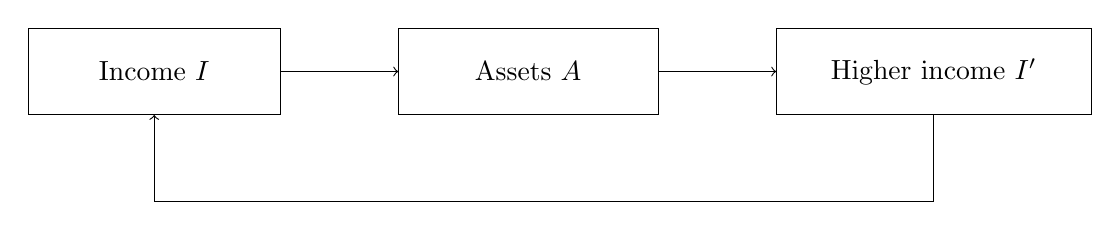
\begin{tikzpicture}
\draw (0,0) rectangle (3.2,1.1);
\node at (1.6,0.55) {Income \(I\)};

\draw (4.7,0) rectangle (8.0,1.1);
\node at (6.35,0.55) {Assets \(A\)};

\draw (9.5,0) rectangle (13.5,1.1);
\node at (11.5,0.55) {Higher income \(I'\)};

\draw[->] (3.2,0.55) -- (4.7,0.55);
\draw[->] (8.0,0.55) -- (9.5,0.55);
\draw[->] (11.5,0) -- (11.5,-1.1) -- (1.6,-1.1) -- (1.6,0);
\end{tikzpicture}
\caption{The reinvestment loop: get money, then buy income.}
\end{figure}

Next comes a ranking principle. Victor says time is worth more than money. It is better to read this not as a market price claim but as an ordering of strategic priorities:
\begin{equation}
\text{time} \succ \text{money},
\end{equation}
where \(\succ\) means ``takes priority over'' rather than ``is numerically larger than.'' The point is that wealth depends on what time is spent on. Attractive distractions are cheap in the short run and expensive in the long run; boring, simple, repeatable work often has the opposite profile.

The lecture then identifies social media marketing as the most important skill for a young entrepreneur trying to move from zero to one million. This belongs naturally with the earlier discussion of attention. The reason is not mysterious. If the early game is a struggle for visibility, then marketing is the operational skill that purchases visibility without necessarily buying expensive media.

Finally, the interviewer applies a stress test. Suppose everything is taken away and the bank account returns to zero. What is the first move? Victor's answer is procedural rather than grand:
\begin{enumerate}
\item Use the network to secure a small funding base, stated here as \(\$10{,}000\).
\item Start a fast cash-flow business, such as car detailing.
\item Stack funds and keep the hands busy.
\item Re-enter higher-leverage digital business only after cash flow is restored.
\end{enumerate}

This is important because it reveals what the lecture thinks is portable. The portable part is not a single lucky business. The portable part is the sequence: network, immediate cash flow, disciplined reinvestment, and then return to scale.

The final question in the interview shifts from mechanism to remembrance. Victor says he wants a wider reach and wants to be known for helping other people change their financial trajectory. That closing matters. It tells us that the technical material of the lecture is not intended to end in private accumulation alone; it is meant to travel outward into reputation, instruction, and example.

\section{Summary}

We can now state the chapter's logic in a compact form. First, large wealth targets are made manageable by decomposition:
\[
T = u \cdot n.
\]
Second, attention is accumulated by cadence rather than by waiting for perfection. Third, sales improve when pressure is reduced and status, quality, and scarcity reverse the direction of pursuit. Fourth, network matters because environment changes the working ceiling. Fifth, money is not merely spent; it is turned back into income-producing assets:
\[
I \to A \to I', \qquad I' > I.
\]

What began as a success profile thus turns into a small theory of entrepreneurial motion. We proceed one figure at a time, we remain in front of people, we enter rooms with value, and we cycle income back into future income. That is the lecture's arithmetic of scale.